\documentclass[review]{elsarticle}

\usepackage{lineno,hyperref}
\usepackage{amsmath}
\usepackage{graphicx}
\usepackage{amsfonts}
\usepackage{booktabs}
\usepackage{subcaption}
\usepackage[section]{placeins}
\usepackage[utf8]{inputenc}

\modulolinenumbers[5]

% \journal{Journal of \LaTeX\ Templates}

%%%%%%%%%%%%%%%%%%%%%%%
%% Elsevier bibliography styles
%%%%%%%%%%%%%%%%%%%%%%%
%% To change the style, put a % in front of the second line of the current style and
%% remove the % from the second line of the style you would like to use.
%%%%%%%%%%%%%%%%%%%%%%%

%% Numbered
%\bibliographystyle{model1-num-names}

%% Numbered without titles
%\bibliographystyle{model1a-num-names}

%% Harvard
%\bibliographystyle{model2-names.bst}\biboptions{authoryear}

%% Vancouver numbered
%\usepackage{numcompress}\bibliographystyle{model3-num-names}

%% Vancouver name/year
%\usepackage{numcompress}\bibliographystyle{model4-names}\biboptions{authoryear}

%% APA style
%\bibliographystyle{model5-names}\biboptions{authoryear}

%% AMA style
%\usepackage{numcompress}\bibliographystyle{model6-num-names}

%% `Elsevier LaTeX' style
\bibliographystyle{elsarticle-num}
%%%%%%%%%%%%%%%%%%%%%%%

\begin{document}

\begin{frontmatter}

\title{Suavização de Malhas não Estruturadas usando-se o Algoritmo Genético}
% \tnotetext[mytitlenote]{Fully documented templates are available in the elsarticle package on \href{http://www.ctan.org/tex-archive/macros/latex/contrib/elsarticle}{CTAN}.}

%% Group authors per affiliation:
\author{Luciano Kiyoshi Araki}
\author{Elton Fernando Doehnert}
% \address{Radarweg 29, Amsterdam}
% \fntext[myfootnote]{Since 1880.}

% % or include affiliations in footnotes:
% \author[mymainaddress,mysecondaryaddress]{Elsevier Inc}
% \ead[url]{www.elsevier.com}

% \author[mysecondaryaddress]{Global Customer Service\corref{mycorrespondingauthor}}
% \cortext[mycorrespondingauthor]{Corresponding author}
% \ead{support@elsevier.com}

% \address[mymainaddress]{1600 John F Kennedy Boulevard, Philadelphia}
% \address[mysecondaryaddress]{360 Park Avenue South, New York}

\begin{abstract}
% Dummy abstract text - replace \blindtext with your abstract text
% This paper presents a method for optimizing a unstructured triangular mesh using a genetic algorithm to find the best position of the nodes of the mesh. This position is based in a fitness of the node that can be changed acoording to some particular need. This algorithm is compared against some other methods and the results shows that the genetic algorithm is able to handle non-convex regions.
A suavização de malhas não-estruturadas é um tópico já muito estudado pois apresenta um impacto muito grande na acurácia da solução numérica em problemas envolvendo o método de elementos finitos e o método de volumes finitos. Esse artigo apresenta um método para otimização de malhas não estruturadas triangulares usando-se um algoritmo genético de ponto flutuante para encontrar a melhor posição para os vértices da malha. Esta posição é baseada na função \textit{fitness} calculada para cada vértice interno à malha, tal função é baseada na média da qualidade dos volumes que compartilham o vértice. O algoritmo é executado para uma malha gerada com triangulação de Delaunay e os resultados mostram que houve uma melhoria na malha com relação ao parâmetro de qualidade estabelecido, no entanto, o método se mostra computacionalmente mais caro que outros métodos de suavização.
\end{abstract}

\begin{keyword}
Algoritmo Genético \sep Evolução \sep Malha não estruturada \sep Suavização
% \MSC[2010] 00-01\sep  99-00
\end{keyword}

\end{frontmatter}

\linenumbers

\section{Introdução}

Embora ferramentas de geração de malhas automáticas sejam amplamente usadas, essas ferramentas podem não garantir a qualidade das malhas. Não apenas no processo de tesselação, mas também no refinamento da malha, é possível que alguns elementos severamente distorcidos ou fora de forma sejam criados. Mesmo quando uma malha uniforme é desejada, a ferramenta de tesselação pode gerar elementos que são muito pequenos ou muito grandes comparados com os elementos desejados. \cite{Zhou}

Existem vários tipos de esquemas de suavização de malhas, tais como suavização Laplaciana e suavização baseada em otimização. Tipicamente cada método possui um compromisso entre qualidade e custo computacional. Por exemplo, a suavização Laplaciana requer um custo computacional muito baixo, mas frequentemente resulta em uma malha de baixa qualidade nos elementos ou mesmo com elementos inválidos. Por outro lado, enquanto suavizações baseados na otimização são mais prováveis em evitar elementos inválidos e obtém uma maior qualidade na malha, o custo computacional é muito maior que a suavização Laplaciana. \cite{Zhou}

Algoritmos Genéticos (GAs) são métodos adaptativos que podem ser usados para resolver problemas envolvendo procura e otimização. Eles são baseados nos processos genéticos de organismos biológicos. Ao longo de muitas gerações, populações naturais evoluem de acordo com os princípios da seleção natural e "sobrevivência do mais apto", primeiramente pronunciados por Charles Darwin no livro \textit{A Origem das Espécies}. Imitando este processo, o algoritmo genético é capaz de "evoluir" soluções para problemas do mundo real, desde que tenham sido corretamente codificados. Por exemplo, GAs podem ser usados para desenhar estruturas de pontes, para a maior proporção de força/peso, ou para determinar a menor quantidade de sobras no corte de tecidos. Ele também pode ser usado para o controle de processos online, tais como em uma fábrica química, ou balanceando sistemas de computadores de multi processadores. \cite{Beasley1993}

O GA usa uma analogia direta com a natureza, onde indivíduos de uma população, representados no algoritmo por possíveis soluções de um problema, recebem um nível de adaptabilidade de acordo com a sua performance na solução do problema, tal nível é denominado \textit{fitness}. Indivíduos com um alto valor de \textit{fitness} possuem uma maior probabilidade para se reproduzirem, ou seja, passarem suas características para a nova população. Já membros da população bom baixo \textit{fitness} irão ter menor chance de reprodução, de modo que ao longo do tempo terão suas características genéticas extintas.

No algoritmo genético, uma solução em potencial para o problema pode ser representado por um conjunto de parâmetros. Esses parâmetros (conhecidos como \textit{genes}) são unidos juntos para formar uma cadeia de valores (frequentemente chamados de \textit{cromossomos}). (\cite{Holland1992} foi o primeiro a mostrar e muitos ainda acreditam que o ideal é o uso de um alfabeto binário para essa cadeia de valores.) Por exemplo, se nosso problema for o de maximizar uma função de três variáveis, $F(x,y,z)$, nós podemos representar cada variável por um número binário de 10-bits. Nossos cromossomos, portanto, conteriam três genes, e possuiriam 30 números binários. No entanto, segundo \cite{Janikow1991} pode-se representar essas variáveis usando-se uma codificação de ponto flutuante, e com essa representação o algoritmo se torna mais rápido, mais consistente e com maior precisão especialmente em domínios grandes, em que a codificação binária se tornaria demasiadamente longa.

Em termos genéticos, o conjunto de parâmetros representados por um dado cromossomo é chamado de \textit{genótipo}. O genótipo contém informações necessárias para construir um organizmo - que é chamado de \textit{fenótipo}.

\section{Métodos}

O método utilizado consiste na geração de uma malha usando-se triangulação de Delaunay conformada, método que gera triangulações de alta qualidade. Este método é descrito em \cite{Shewchuk2002} e \cite{Lin1996}. Esta malha é, então, otimizada utilizando-se o algoritmo genético em cada um de seus vértices internos, se modo a se estabelecer a melhor posição com relação a um critério de qualidade, essa qualidade é definida em \cite{Falsafioon2014} e é calculada para cada volume da malha conforme a equação:

\begin{equation}
    SQ_i = \frac{4 \sqrt{3} A_i}{\sum_{i=1}^3 l_i^2}
    \label{eq:01}
\end{equation}

No problema da determinação da posição ideal dos vértices da malha, pode-se definir um conjunto de coordenadas cartesianas para a determinação dessa posição, tal conjunto pode ser denominado pelo \textit{genótipo} da solução enquanto que o \textit{fenótipo} é a média da qualidade dos volumes que compartilham esse vértice. A adaptação de cada indivíduo depende da performance do seu fenótipo. Isso pode ser inferido do seu \textit{genótipo} - i.e. pode ser computado do seu cromossomo usando a função fitness.

\subsubsection{Algoritmo}

Cada geração será definida por uma nova população, que irá ter, em média, um melhor \textit{fitness} médio e irá, portanto, convergir para uma solução do problema. Um resumo da metodologia usando-se algoritmo genéticos é dada por \cite{Kumar2010} e é dada por:
\begin{itemize}
    \item \textbf{Inicialização:} Inicialmente muitas soluções representando indivíduos são geradas aleatoriamente de modo a se formar a população inicial. O tamanho dessa população depende da natureza do problema, mas tipicamente contém muitas centenas de milhares de possíveis soluções. Tradicionalmente, a população é gerada aleatoriamente, cobrindo-se todo o possível espaço de soluções. Ocasionalmente, pode-se priorizar determinada área desse espaço entendido como tendo uma maior probabilidade de ter a solução ideal.
    \item \textbf{Seleção:} A cada nova geração, um conjunto da população atual é selecionada de alguma forma de modo a gerarem a nova geração. Tais indivíduos são selecionados pela sua função \textit{fitness}. Alguns métodos calculam o fitness de toda a geração enquanto outros selecionam apenas alguns indivíduos aleatórios, no entanto este último método pode ser muito mais custoso com relação ao tempo.
    Normalmente a função fitness escolhida é estocástica e feita de tal forma que mesmo soluções com baixo fitness tem uma pequena chance de serem selecionadas, tal estratégia ajuda a manter a diversidade genética da população alta, prevenindo o surgimento prematuro de soluções ruins. As formas de seleção mais estudadas e usadas incluem seleção \textit{roulette whell} e \textit{tournament selecion}.
    \item \textbf{Reprodução:} O próximo passo é a geração dos novos indivíduos que irão fazer parte da nova população, que irá substituir a população antiga. Tal reprodução é feita usando-se o \textit{genótipo} dos pais selecionados e os recombinando através do processo de \textit{crossover} e \textit{mutation}.
    Como a "criança" gerada nesse processo possui genótipos dos dois pais, ela compartilhará muitas características com seus "pais". Novos pais são selecionados para cada nova criança e esse processo continua até toda a nova população ser gerada. Embora tipicamente escolham-se apenas dois pais para cada criança, alguns pesquisadores \cite{Eiben2012} sugerem que mais de dois pais podem produzir uma criança com um melhor genótipo.
\end{itemize}

O processo de evolução de novas soluções(indivíduos) continua até que algum critério de parada seja estabelecido, que pode ser:
\begin{itemize}
    \item Uma solução é encontrada satisfazendo um critério mínimo;
    \item Um número de gerações fixado é alcançado;
    \item Um tempo computacional é alcançado;
    \item A solução com o maior fitness da população atinge um platô tal que novas gerações não conseguem melhorar o resultado;
    \item Inspeção Manual;
    \item Uma combinação das anteriores.
\end{itemize}

% \subsection{Suavização \textit{Centroidal Voronoi Tessellation}}

% O método \textit{centroidal Voronoi tesselation} é uma tesselação cujos pontos gerados são os centróides das regiões de Voronoi correspondentes. \cite{Du1999}

% Dado um conjunto aberto $\Omega \subset \mathbb{R}^N$, o conjunto ${V_i}_{i=1}^k$ é chamado de uma tesselação de $\Omega$ se $V_i \cap V_j = \emptyset$ para $i \neq j$ e $\cup_{i=1}^k \hat{V_i} = \hat{\Omega}$.

% Dado um conjunto de pontos ${z_i}_{i=1}^k$ pertencentes a $\hat{\Omega}$, a região de Voronoi $\hat{V_i}$ que corresponde aos pontos $z_i$ é definida por:

% \begin{equation}
%     \hat{V_i} = {x \in \Omega |  |x-z_i| < |x-z_j| \text{para} j=1,...,j, j \neq i }
% \end{equation}

% Os pontos ${z_i}_{i=1}^k$ são chamados de sementes. Enquanto que o conjunto ${\hat{V_i}}_{i=1}^k$ é chamado de diagrama de Voronoi de $\Omega$ e cada $\hat{V_i}$ se refere a região de Voronoi correspondente a $z_i$.

% Pode-se entender um diagrama de Voronoi como um conjunto de células em que as fronteiras dessas células estão de tal forma que os pontos contidos nas células são os mais próximos de um ponto específico. Ou seja, um diagrama de Voronoi é uma maneira de particionar um plano em regiões conhecidas como células baseado na distância de um conjunto específico de pontos conhecidos como sementes. Cada célula possui uma semente e os pontos nessa célula estão mais próximos dessa semente do que qualquer outra semente. Além disso pode-se considerar as regiões de Voronoi como poliedros.

% Dado uma região $V \subset \mathbb{R}^N$ e uma função densidade $\rho$, definida em $V$, o centróide de massa $z^*$ de $V$ é definido como:

% \begin{equation}
%     z^* = \frac{\int_V y \rho(y) dy}{\int_V \rho(y) dy}
% \end{equation}

% Dado $k$ pontos $z_i$, $i=1,...,k$ podemos definir as suas regiões de Voronoi associadas $\hat{V_i},i=1,...,k$. Por outro lado, dados as regiões $\hat{V_i},i=1,...,k$ podemos definir seus centros de massa $z_i^k,i=1,...,k$. Nesse caso, interessa a situação em que:

% \begin{equation}
%     z_i = z_i^*, i=1,...,k
% \end{equation}

% Ou seja, os pontos $z_i$ que servem como as sementes (ou geradores) das regiões de Voronoi $\hat{V_i}$ são também os centros de massa dessas regiões. Chama-se tal tesselação como "centroidal Voronoi tessellation".

\section{Resultados}

O algoritmo de otimização baseado no métodos apresentado é implementado para duas geometrias complexas e os resultados estão apresentados nas figuras \ref{fig:malha1} e \ref{fig:malha2}, também é informado para cada malha os valores do maior ângulo, menor ângulo, desvio padrão entre os ângulos, maior qualidade entre os volumes, menor qualidade, desvio padrão da qualidade e a média da qualidade, que pode ser usado como um parâmetro da qualidade geral de uma malha.

\begin{figure}[]
    \begin{subfigure}{1\textwidth}
        \centering
        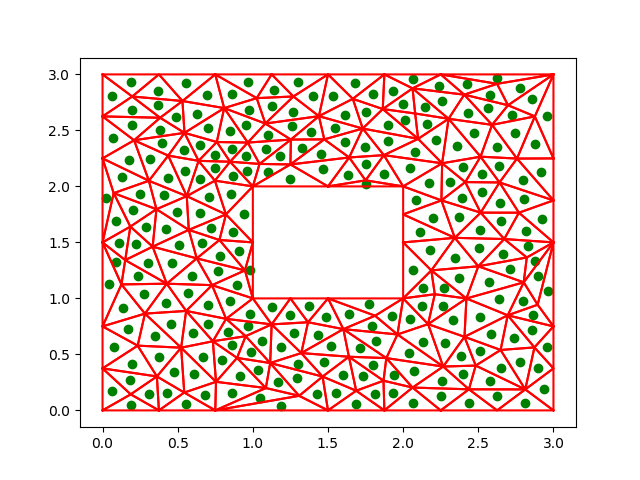
\includegraphics[width=1\textwidth]{malha1-original.png}
        \caption{Malha Original}
        \label{fig:malha-original}
    \end{subfigure}
    \begin{subfigure}{1\textwidth}
        \centering
        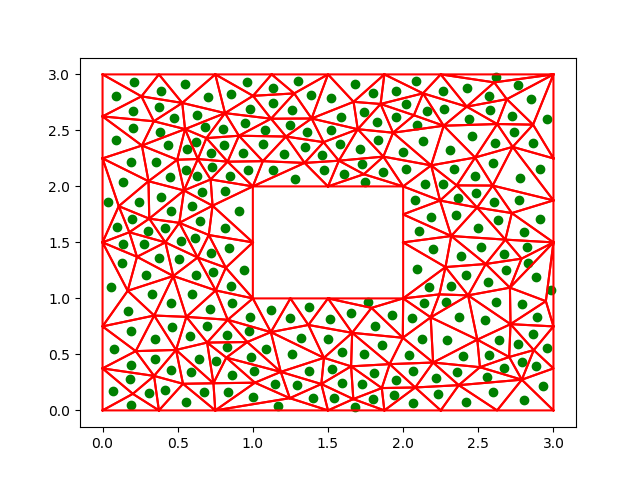
\includegraphics[width=1\textwidth]{malha1-ga.png}
        \caption{Malha após GA}
        \label{fig:malha-ga}
    \end{subfigure}

    \caption{Malha 1}
    \label{fig:malha1}
\end{figure}


\begin{table}[hb]
    \caption{Malha 1 original}
    \centering
    \begin{tabular}{lll}
    \toprule
    Valor & Ângulo & Qualidade \\
    \midrule
    Média & 60 & 0.830759 \\
    Desvio Padrão & 22.868034 & 0.193268 \\
    Mínimo & 9.554770 & 0.076371 \\
    Máximo & 157.010795 & 0.999923
    \end{tabular}
    \label{tb:malha-1-original}
\end{table}

\begin{table}[]
    \caption{Malha 1 com GA}
    \centering
    \begin{tabular}{lll}
    \toprule
    Valor & Ângulo & Qualidade \\
    \midrule
    Média & 60 & 0.848804 \\
    Desvio Padrão & 21.527223 & 0.189446 \\
    Mínimo & 5.504031 & 0.041763 \\
    Máximo & 161.853212 & 0.999185
    \end{tabular}
    \label{tb:malha-1-ga}
\end{table}

\begin{figure}[]
    \begin{subfigure}{1\hsize}
        \centering
        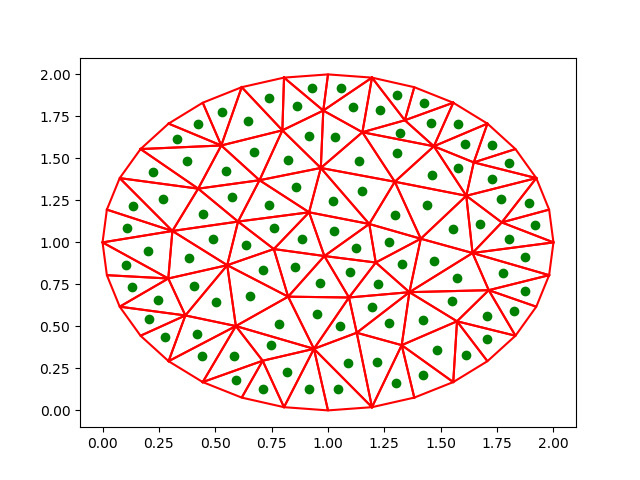
\includegraphics[width=1\textwidth]{malha2-original.png}
        \caption{Malha Original}
        \label{fig:malha-original}
    \end{subfigure}
    \begin{subfigure}{1\hsize}
        \centering
        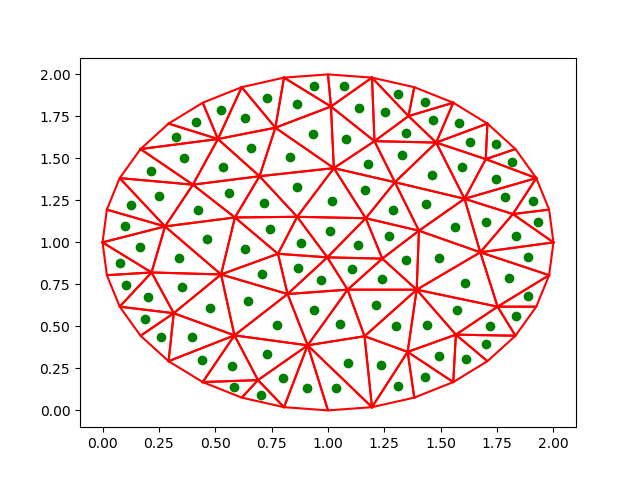
\includegraphics[width=1\textwidth]{malha2-ga.png}
        \caption{Malha após GA}
        \label{fig:malha-ga}
    \end{subfigure}

    \caption{Malha 2}
    \label{fig:malha2}
\end{figure}

\begin{table}[]
\caption{Malha 2 original}
\centering
\begin{tabular}{lll}
\toprule
Valor & Ângulo & Qualidade \\
\midrule
Média & 60 & 0.873503 \\
Desvio Padrão & 17.606637 & 0.102456 \\
Mínimo & 26.888982 & 0.604936 \\
Máximo & 109.030637 &0.999390
\end{tabular}
\label{tb:malha-2-original}
\end{table}

\begin{table}[]
\caption{Malha 2 com GA}
\centering
\begin{tabular}{lll}
\toprule
Valor & Ângulo & Qualidade \\
\midrule
Média & 60 & 0.900385 \\
Desvio Padrão & 15.643499 & 0.098648 \\
Mínimo & 24.665694 & 0.621293 \\
Máximo & 106.827269 & 0.998796
\end{tabular}
\label{tb:malha-2-ga}
\end{table}

\section*{Conclusão}
A otimização de malhas não estruturadas é de grande importância em certos tipos de aplicações, esta otimização pode ser feita com o uso de algum tipo de heurística.

Neste trabalho duas malhas não estruturadas triangulares foram geradas usando-se a triangulação de Delaunay, foi desenvolvido um método baseado no algoritmo genético que otimizasse a posição dos vértices internos da malha baseado em um fator de qualidade. Os resultados mostram que mesmo para uma malha gerada pela triangulação de Delaunay, que é um método muito eficiente de geração de malhas triangulares, o algoritmo foi capaz de melhorar a média da qualidade dos volumes dessa malha, conforme pode ser verificados nas tabelas \ref{tb:malha-1-ga} e \ref{tb:malha-2-ga} em que a qualidade é medida através de um fator de qualidade definido em \ref{eq:01}.

Apesar do algoritmo conseguir melhorar a qualidade das malhas, sabe-se que outros métodos de suavização são mais eficientes em relação ao custo computacional assim como geram um resultado melhor.


\bibliography{referencias}

\end{document}